\pagebreak
\section{Visualization of Time-Oriented and Network Data}
\label{sub:lr-time-network}

\subsection{Time-Oriented Data Visualization}
Many visualization techniques have been developed to explore the temporal relationships of data. The book by Aigner~et~al.~\cite{Aigner2011} provides a comprehensive review of this topic. It discusses the characteristics of time and time-oriented data (what), the tasks aimed to support (why), and the visual representations of time and data (how). The book also reviews interaction and analytical supports for such visualizations. In this section, we briefly describe different visual mappings of time (as summarized in \autoref{fig:lr-time}) and recommend readers to Aigner~et~al.~'s book for further detail.

\begin{figure}[p]
	\centering
	\subcaptionbox{Horizontal axis: Joseph Priestley's Chart of Biography. \is{Priestley1765}
	\label{fig:lr-time-horizontal}}{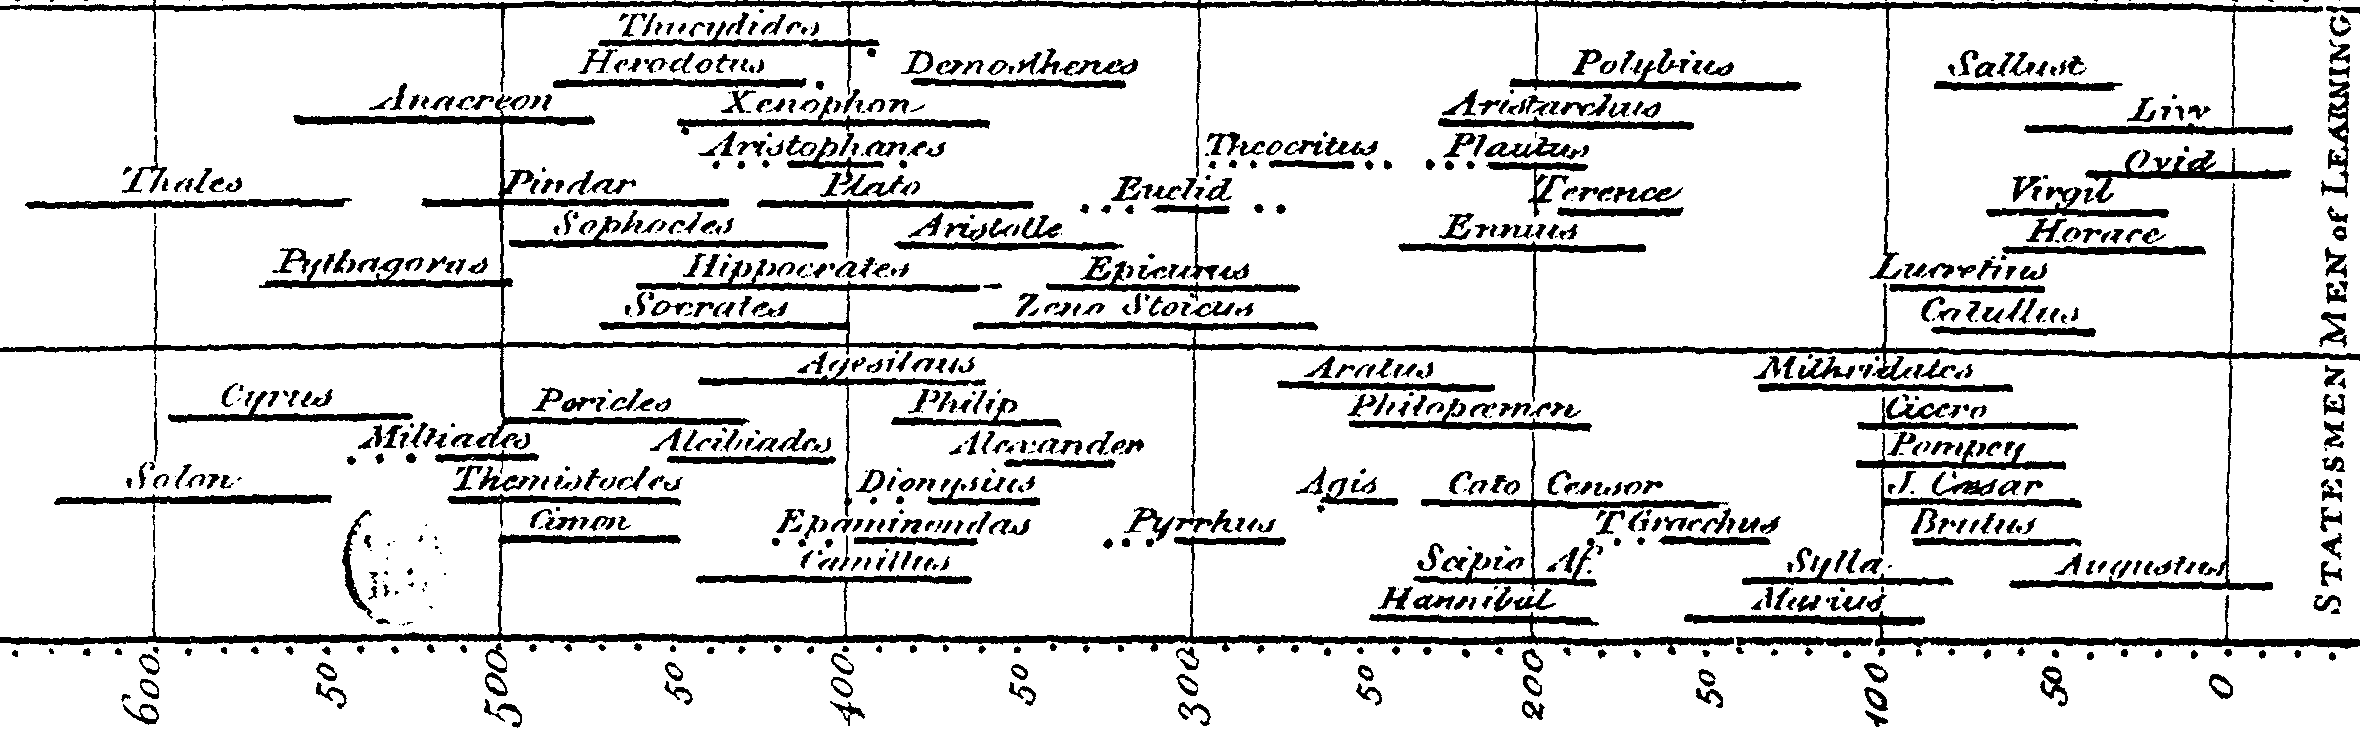
\includegraphics[width=\columnwidth]{biography-chart-crop}}
	\\ \vspace{.5\baselineskip}
	\subcaptionbox{Spiral axis showing two variables (yellow and red). \is{Weber2001} \label{fig:lr-time-spiral}}[.47\columnwidth]{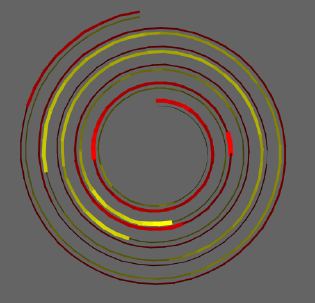
\includegraphics[height=.35\columnwidth]{spiral}}
	\hfill
	\subcaptionbox{Circle axis showing six variables over ten time steps. \is{Keim2004}
	\label{fig:lr-time-circle}}[.47\columnwidth]{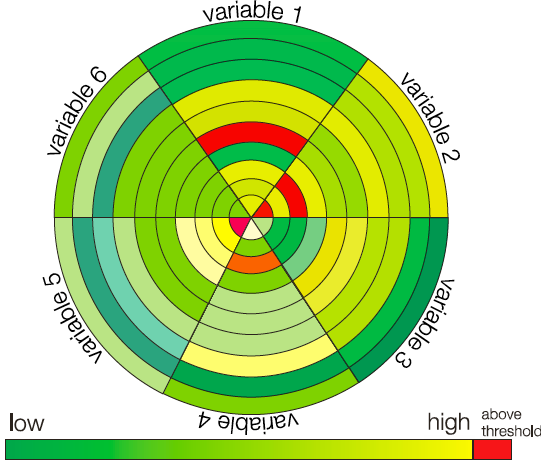
\includegraphics[height=.35\columnwidth]{circle-view}}
	\\ \vspace{.5\baselineskip}
	\subcaptionbox{Calendar visualization of 6-month daily power consumption. \is{VanWijk1999} \label{fig:lr-time-calendar}}{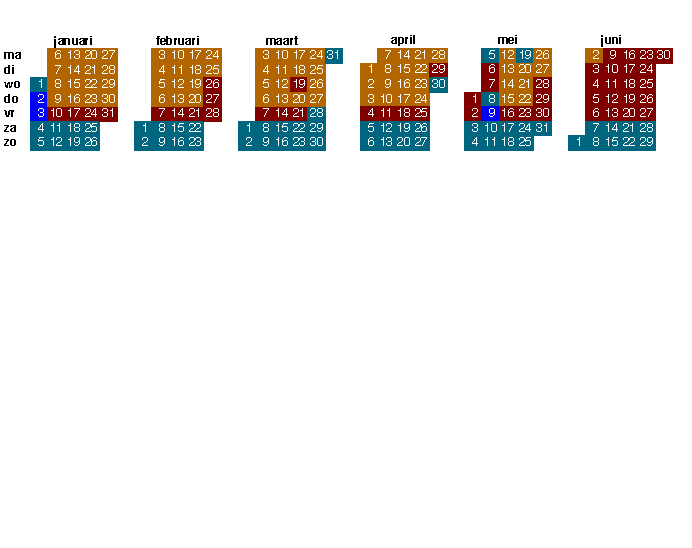
\includegraphics[width=\columnwidth]{calendar-crop}}
	\\ \vspace{.5\baselineskip}
	\subcaptionbox{Small multiples of bar charts showing values from 2001 to 2011. \textit{Image source: \url{https://projects.propublica.org/graphics/ambulances}.} \label{fig:lr-time-multiples}}{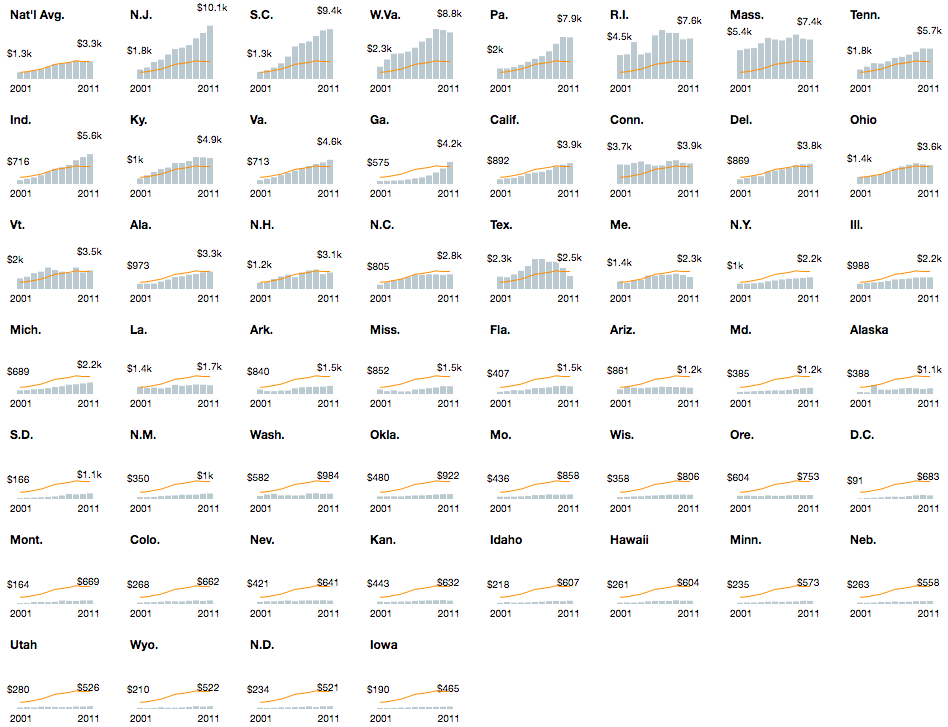
\includegraphics[width=\columnwidth]{small-multiples}}
	\caption{Visual mappings of time.}
	\label{fig:lr-time}
\end{figure}

\subparagraph{Horizontal} Data items are positioned along a horizontal axis as either a point mark for point-based time or a line mark for interval-based time. This is the most common method, and was used in one of the oldest documented timelines -- the \emph{Chart of Biography} by Joseph Priestley~\cite{Priestley1765} back in 1765 -- as shown in \autoref{fig:lr-time-horizontal}. It displays the lifespans of famous people along a horizontal time axis, using a line segment to depict a lifespan, and dots to indicate uncertain values.

\subparagraph{Spiral} Data can be positioned along a spiral axis~\cite{Weber2001}. Color intensity and line thickness are suitable for encoding an additional quantitative variable. Spirals can also be intertwined to show multiple variables. \autoref{fig:lr-time-spiral} shows a spiral graph comparing two variables over time with different color hues.

\subparagraph{Circle} A circle-based approach can be used to visualize time-related multidimensional datasets~\cite{Keim2004}. A circle is split into multiple concentric rings, each for a time step; and is divided into a number of sectors, each representing a variable. \autoref{fig:lr-time-circle} shows such a visualization with six variables.

\subparagraph{Calendar} This method color-codes days in a calendar based on value of a data attribute to reveal patterns at different temporal granularities such as daily, weekly and monthly~\cite{VanWijk1999}. \autoref{fig:lr-time-calendar} visualizes the daily power consumption over a year with color indicating the result of a clustering algorithm.

\subparagraph{Small Multiples}  Miniature data visualization at different time points can be positioned next to each other to facilitate overview and comparison. This method can be applied to all static visualizations because only small screen shots of the visualization for each time step are required. \autoref{fig:lr-time-multiples} shows small multiples of bar charts.

\subparagraph{Animation} This is another time mapping that can be applied to all static visualizations. It relies on human perception in perceiving changes while a visualization smoothly updates from one time step to another~\cite{Gapminder}. Only a few data items should be animated, and they are often highlighted so that users can keep track of the changes.

\paragraph{Summary} Horizontal time axis is a conventional mapping and easy to understand, whereas spiral time axis is good at detecting cyclic patterns. Calendar is another user-friendly representation and can reveal patterns at different granularities. Animation can be an appealing choice for presentation, but it is both slower and less accurate than small multiples in conveying trends over time~\cite{Robertson2008}. In this thesis, \autoref{chap:schemaline} contributes a novel timeline visualization that is inherently designed for sensemaking and based on horizontal time axis mapping. \autoref{chap:timesets} extends the technique to support making sense of complex relationships by showing both temporal and categorical information simultaneously.

\subsection{Network and Tree Data Visualization}
Network visualization is an established research topic with many comprehensive survey papers such as~\cite{Herman2000}. A more recent survey published in 2011 by Landesberger et~al.~\cite{Landesberger2011}. It discusses visual representations of network data together with interaction and analysis techniques. In this section, we briefly describe common methods in visualizing network and tree data (as summarized in \autoref{fig:lr-network}) and recommend readers to aforementioned surveys for further detail.

\begin{figure}[t]
	\centering
	\subcaptionbox{Matrix view with gray cells showing connectivity. \is{Munzner2014} \label{fig:lr-network-nodelink}}[.45\columnwidth]{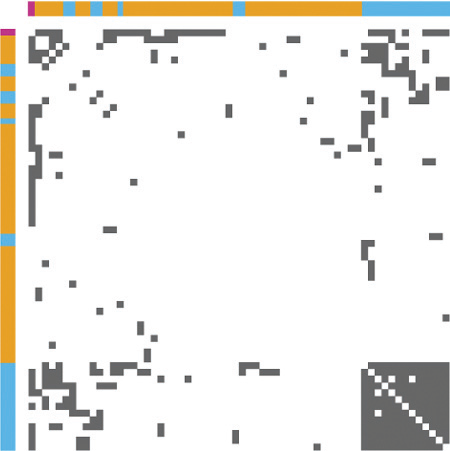
\includegraphics[height=.4\columnwidth]{matrix-2}}
	\hfill
	\subcaptionbox{Force-directed graph with links showing connectivity. \is{Munzner2014} \label{fig:lr-network-matrix}}[.49\columnwidth]{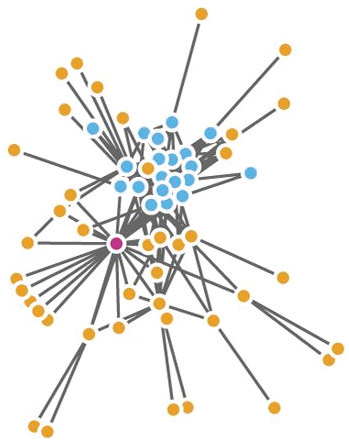
\includegraphics[height=.4\columnwidth]{matrix-3}}
	\\ \vspace{.5\baselineskip}
	\subcaptionbox{Treemap showing the class hierarchy of the Flare visualization toolkit~\cite{Heer2009b}. Area represents class sizes and color represents the top-level classes. \textit{Image source: \url{https://bl.ocks.org/mbostock/4063582}.} \label{fig:lr-network-treemap}}{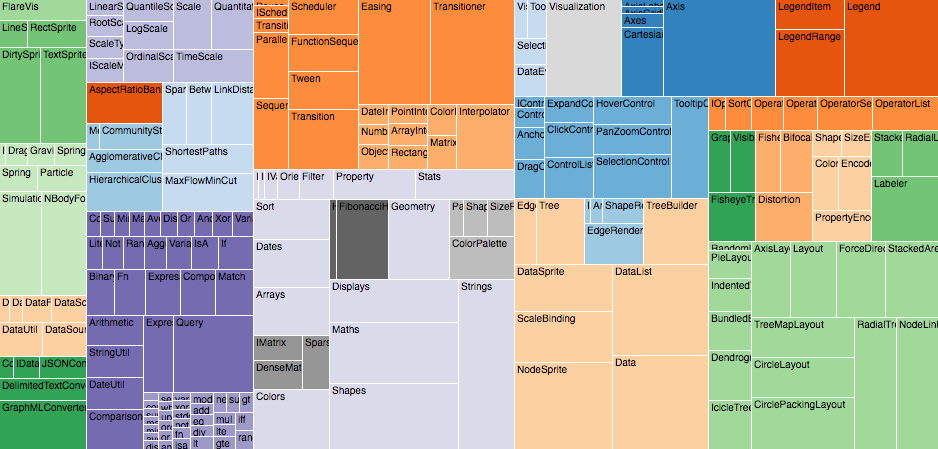
\includegraphics[width=\columnwidth]{treemap}}
	\caption{Visual representations of network and tree data.}
	\label{fig:lr-network}
\end{figure}

\subparagraph{Node-Link Diagrams}
This is the most common visual encoding for network and tree data, where nodes are represented as \emph{point} marks and links connecting these nodes are represented as \emph{connection} marks. Force-directed layout~\cite{Eades1984} is often used to generate an aesthetically pleasing output based on a simulation of physical forces.  \autoref{fig:lr-network-nodelink} shows an example of a medium-size network.

\subparagraph{Matrix Views}
A network can be represented by an adjacency matrix. Each row and column of the matrix corresponds to a node, and a cell indicates whether the pair of corresponding nodes is connected in the network. Additional information about edges can be encoded to the visual representation of cells using color, shape and size. \autoref{fig:lr-network-matrix} shows an example of matrix view using the same dataset as in \autoref{fig:lr-network-nodelink}.

\subparagraph{Space-Filling Techniques}
Space-filling techniques can only be applied to tree data and uses \emph{containment} marks to represent hierarchical relationship, placing child nodes within their parent node. Treemap~\cite{Shneiderman1992} represents a node as a rectangle, which is recursively subdivided into smaller rectangles, each representing a child of the node. The rectangle size is proportional to a quantitative attribute of its node. \autoref{fig:lr-network-treemap} shows an example of treemap.

\paragraph{Summary}
Node-link diagrams are user-friendly and suitable for small datasets, whereas matrix views are better at large datasets~\cite{Ghoniem2005}. Space-filling techniques produce a compact visualization of tree data and are effective in using size to represent a quantitative attribute. \autoref{chap:sensemap} also uses network data showing pair-wise relationships between provenance data items. Even though it applies an existing tree layout, the research discussed in this section lays the foundation for making suitable design decisions. To address scalability, our tree visualization includes representations for different levels of detail and interactive features such as semantic zooming and panning.